% !TeX spellcheck = de_DE

%  ******************************************************************************
%  * @file      LatexVorlageMH                                                  *
%  * @author    Mario Hesse                                                     *
%  * @version   v2.0.1                                                          *
%  * @date      31.01.2019                                                      *
%  * @brief     Vorlage für wissenschaftliche Arbeiten.                         *
%  *            Erstellt von Mario Hesse                                        *
%  *                                                                            *
%  *            Alle Kapitel, die Präambel, Bilder, Literatur, etc. sind in     *
%  *            einzelnen Ordnern hinterlegt. Dadurch entsteht mehr Übersicht   *
%  *            und Ordnung.                                                    *
%  *              - Präambel:   /tex/                                           *
%  *              - Glossar:    /tex/                                           *
%  *              - Kapitel:    /tex/                                           *
%  *              - Bilder:     /pic/                                           *
%  *              - Daten:      /dat/                                           *
%  *              - Anhang:     /app/                                           *
%  ******************************************************************************

% Alle Dateien mit den nachfolgenden Endungen sind Hilfsdateien und können regelmäßig gelöscht werden. Dadurch können Fehlerhafte Dokumente oft wieder Lauffähig werden. 
% log, aux, dvi, lof, lot, bit, idx, glo, bbl, bcf, ilg, toc, ind, out, blg, fdb_latexmk, fls, acn, acr, alg, glg, gls, ist, slg, syg, syi, synctex.gz, tdo


% !TeX spellcheck = de_DE

%  ******************************************************************************
%  * @file      tex/preamble                                                    *
%  * @author    Mario Hesse                                                     *
%  * @version   v0.1.1                                                          *
%  * @date      16.10.2019                                                      *
%  ******************************************************************************



% ******************************************************************************
% Dokument / Seiten
% ******************************************************************************

\documentclass[12pt,a4paper,parskip=full+]{scrartcl}
\usepackage[utf8]{inputenc}														% Zeichencodierung
\usepackage[ngerman,english]{babel}												% Sprachpaket Deutsch ausgewählt
\selectlanguage{ngerman}														% Sprache auf Deutsch gesetzt
\usepackage[T1]{fontenc}														% Umlaute bei \hyphenation verwenden können (Silbentrennung)
\usepackage[onehalfspacing]{setspace}											% Setzt das Dokument auf 1,5x Zeilenabstand (singlespacing/onehalfspacing/doublespacing)
\usepackage[headsepline]{scrlayer-scrpage}										% Kopfzeile
\usepackage[defaultlines=4,all]{nowidow}										% Schusterjungen und Hurenkinder
\usepackage{																	% Standard Krempel
	amsmath,																	% American Mathematical Society - Mathematik Basics (equation, equation*, align, align*, gather, gather*, flalign, flalign*, multline, multline*, alignat, alignat*, ...)
	amsfonts,																	% Schriftarten für Mathematik und spezielle Symbole
	amsthm,																		% erlaubt die Definition von Theoremen
	amssymb}																	% mathematische Zeichen und Symbole
\usepackage[version=4]{mhchem}													% erlaubt Chemische Gleichungen | bsp. \ce{C6H12O6 + 6O2 -> 6CO2 + 6H2O}



% ******************************************************************************
% Verlinkungen & Metadaten
% ******************************************************************************

\usepackage[																	% Verlinkung aller sections, ref , url, etc.
pdfborderstyle={/S/U/W 1}														% ändert den Rahmen der Links in Unterstriche
% colorlinks=true,																% schaltet Rahmen um die Links aus und ändert stattdessen die Schriftfarbe
% urlcolor=blue,																% URL Links: Blau
% citecolor=black,																% Zitate: Schwarz
% linkcolor=black																% Dokumentenlinks: Schwarz
]{hyperref}

\hypersetup{																	% erweiterte Einstellungen zu "hyperref" und erlaubt \autoref{} ist ähnlich wie \ref{}, schreibt aber Abbildung, Tabelle, usw. vor die verlinkte Gleitumgebung)
%	bookmarks=true,																% zeigt die Lesezeichenleiste an oder nicht.
	unicode=true,																% ermöglicht die Verwendung von nicht-latin Schriftzeichen
	pdftoolbar=true,															% setzt den Rahmen um einen Link, {0 0 0} erzeugt keinen Rahmen
	pdfmenubar=true,															% zeigt die Acrobat-Toolbar an oder versteckt sie.
	pdffitwindow=false,															% zeigt das Acrobat-Menü an oder versteckt es.
	pdfstartview={FitH},														% verändert die Größe des Acrobat-Anzeigefensters, damit das Dokument hineinpasst.
	pdftitle={Ein ziemlich guter wissenschaftlicher Arbeitstitel},				% definiert den Titel des Dokuments, welcher in der Dokumenteninfo von Acrobat angezeigt wird.
	pdfauthor={Vorname Name},													% definiert den Namen des Autors für die Dokumenteninfo.
	pdfsubject={},																% Beschreibung des Dokument für die Dokumenteninfo.
	pdfcreator={Vorname Name},													% Ersteller des Dokuments für die Dokumenteninfo.
	pdfproducer={},																% Produzent des Dokuments für die Dokumenteninfo.
	pdfkeywords={Plasma} {Hochschule für angewandte Wissenschaft und Kunst} {HAWK} {Göttingen},		% Schlüsselwörter des Dokuments für die Dokumenteninfo (durch geschweifte Klammern voneinander getrennt).
	pdfnewwindow=true,															% legt fest, dass Links in einem neuen Fenster geöffnet werden sollen.
	colorlinks=false,															% legt fest, ob ein farbiger Rahmen um die Links gezogen werden soll oder ob die Schrift farbig sein soll.
	linkcolor=red,																% Farbe für die Links.
	citecolor=green,															% Farbe für die Quelllinks (bibliography; Quellenverzeichnis).
	filecolor=magenta,															% Farbe für Dateilinks.
	urlcolor=cyan																% Farbe für URL-Links (Web, Mail).
}

\renewcaptionname{ngerman}\sectionautorefname{Abschnitt}						% Ändern von \autoref(section):  Abschnitt           -> Abschnitt
\renewcaptionname{ngerman}\subsectionautorefname{Abschnitt}						% Ändern von \autoref(section):  Unterabschnitt      -> Abschnitt
\renewcaptionname{ngerman}\subsubsectionautorefname{Abschnitt}					% Ändern von \autoref(section):  Unterunterabschnitt -> Abschnitt
\newcommand{\subfigureautorefname}{\figureautorefname}							% Ändern von \autoref(subfloat): Unterabildung      -> Abbildung

\usepackage{cleveref}															% Muss nach \hypreref geladen werden (!) | \cref ist ähnlich wie \autoref, schreibt aber Abb., Tab., usw. vor die verlinkte Gleitumgebung



% ******************************************************************************
% Korrektur- und Dokumentatitonswerkzeuge
% ******************************************************************************
%\usepackage{comment}															% Erlaubt das Verwenden der Umgebung \begin{comment}...\end{comment} -> Erstellen von Kommentaren über mehrere Zeilen
\usepackage[ngerman,
			disable,															% Paket deaktiviert | zum Aktivieren Zeile auskommentieren
			textsize=tiny,														% Todo-Notes werden in der Schriftgröße tiny angelegt
			colorinlistoftodos,													% die Farben der Todo-Notes werden in der List of Todos mit angezeigt
			]{todonotes}														% erlaubt das Verwenden von ToDo-Notizen -> \todo{...} und Blindbildern -> \missingfigure{...}

\usepackage[ngerman]{translator}												% erlaubt anderen Paketen Begriffe in Deutsche zu Übersetzen (Figure -> Abbildung, Table -> Tabelle, etc.)

\setlength{\headheight}{1.1\baselineskip}

\newcommand{\Autor}[2][]{\todo[color=yellow!40,#1]{\textbf{Autor:} #2}}			% neues Kommando \Autor{} (Sollte nach dem Autor benannt werden), um mit mehreren Leuten \todo{} zu nutzen
\newcommand{\KorrektorEins}[2][]{\todo[color=blue!40,#1]{\textbf{Korrektor1:} #2}}	% neues Kommando \Korrektor1{} (Sollte nach dem 1. Korretor benannt werden), um mit mehreren Leuten \todo{} zu nutzen
\newcommand{\KorrektorZwei}[2][]{\todo[color=green!40,#1]{\textbf{Korrektor2:} #2}}% neues Kommando \Korrektor2{} (Sollte nach dem 2. Korretor benannt werden), um mit mehreren Leuten \todo{} zu nutzen

\usepackage{changes}															% Erlaubt Änderungen nachverfolgen \deleted{} \replaced{}{}


% ******************************************************************************
% Gleitumgebungen / Grafiken
% ******************************************************************************

\usepackage{float}																% notwendig für Gleitumgebungen z.B. Figure
\usepackage{graphicx}															% erlaubt das Einbinden von Grafiken
\usepackage{subfig}																% erlaubt das Verwenden von Subfigures (Mehrere Bilder in einer Figure-Umgebung)
\usepackage{wrapfig}															% eröffnet die Möglichkeit Text neben eine Figure zu schreiben
\usepackage{pdfpages}															% ermöglicht das Einbinden von PDFs
\usepackage{epstopdf}															% erlaubt das Einbinden von EPS-Bilddateien
\usepackage{afterpage}															% erlaubt einen Punkt zu definieren, an dem alle bisherigen Floats gezeichnet sein müssen | Anwendung: \afterpage{\clearpage}
\usepackage{listings}															% ermöglicht zeichengenaues Zitieren (für Programmcode) \verb|Zitat|
	\renewcommand{\lstlistingname}{Quelltext}    								% Caption von "Listening" auf "Code" ändern
\usepackage{caption}															% ermöglicht die Beschriftung von Gleitobjekten (Floats)
\usepackage{nameref}															% erlaubt Namensreferenzen


\usepackage{enumitem}															% ermöglicht das Einstellen von Abständen in itemize-Umgebungen -> \setitemize{noitemsep,topsep=0pt,parsep=0pt,partopsep=0pt} (global) oder begin{itemize}[noitemsep,topsep=0pt,parsep=0pt,partopsep=0pt] (lokal) und erlaubt das Verwenden der enumitem-Umgebung (itemize mit geringeren Abständen)
\setitemize{noitemsep,topsep=0pt,parsep=0pt,partopsep=0pt}						% Veringern der Abstände in allen itemize-Umgebung des Dokuments

\usepackage{abstract}															% erlaubt das Verwenden der standartisierten Vorlage für Abstracts ( \begin{abstract}...\end{abstract} )
\addto\captionsngerman{\renewcommand{\abstractname}{Kurzfassung}}				% benennt den deutschen Titel des Abstracts von 'Zusammenfassung' um in 'Kurzfassung' 

\usepackage{forest}																% erlaubt einfache Verzeichnisstrukturen (tree), ist super für Verzeichnisbäume geeignet


% ******************************************************************************
% Tabellen
% ******************************************************************************
\usepackage{tabularx}															% ermöglicht Tabellen mit konkreter Breite festzulegen und erlaubt Zeilenumbrüche in einer Tabelle
\usepackage{longtable}															% lange Tabellen, welche über mehrere Seiten verarbeitet werden können


% Definieren neuer Tabellenspalten-Typen
% --------------------------------------
\newcolumntype{L}[1]{>{\raggedright\arraybackslash}p{#1}} 						% linksbündig mit Breitenangabe -> L{BREITE} statt p{BREITE} möglich
\newcolumntype{C}[1]{>{\centering\arraybackslash}p{#1}} 						% zentriert mit Breitenangabe -> C{BREITE} statt p{BREITE} möglich
\newcolumntype{R}[1]{>{\raggedleft\arraybackslash}p{#1}} 						% rechtsbündig mit Breitenangabe -> R{BREITE} statt p{BREITE} möglich
\newcolumntype{Y}{>{\centering\arraybackslash}X}								% wie X Spalten, aber zentrieren
\newcolumntype{Z}{>{\raggedleft\arraybackslash}X}								% wie X Spalten, aber rechtsbündig

\newcommand{\ltab}{\raggedright\arraybackslash} 								% Tabellenabschnitt linksbündig -> \ltab
\newcommand{\ctab}{\centering\arraybackslash} 									% Tabellenabschnitt zentriert -> \ctab 
\newcommand{\rtab}{\raggedleft\arraybackslash} 									% Tabellenabschnitt rechtsbündig -> \rtab


% Zusätzliche Tabellenfunktionen
% ------------------------------
\usepackage{multirow}															% erlaubt in Tabellen das Zusammenfassen von Zellen in einer Reihe
\usepackage{booktabs}															% erlaubt mehrere unterschiedliche Linien in Tabellen (\toprule, \midrule, \bottomrule)
\usepackage{hhline}																% erlaubt individuelle Dicke bei Tabellenlinien



% ******************************************************************************
% Diagramme
% ******************************************************************************

\usepackage{tikz}																% Zeichentool
\usepackage{pgfplots, pgfplotstable}											% Diagramme zeichnen
\pgfplotsset{compat = newest}													% Einstellung für Diagramme
\usepackage{pgfgantt}                                                           % Gantt-Diagramme zeichnen
\usepackage[binary-units]{siunitx}      										% SI-Einheiten können verwendet werden | Anwendung: \si{\meter\per\second}
\usepgfplotslibrary{units}														% Einheiten in Diagrammen plotten



% ******************************************************************************
% Verzeichnisse
% ******************************************************************************
\usepackage{scrwfile}                                                           % Erlaubt das Erstellen von mehr als 16 Verzeichnissen (Inhaltsverzeichnis, Glossar, ...)

% Literaturverzeichnis
% --------------------
\usepackage[
	backend=biber,
	style=ieee,
	citestyle=numeric
	]{biblatex}
\addbibresource{bib/Literatur.bib}


% Inhaltsverzeichnis
% ------------------
\usepackage{tocstyle}															% toc = Table of Content | Paket für Inhaltsverzeichnis (\tableofcontents), Abbildungsverzeichnis (\listoffigures) und Tabellenverzeichnis (\listoftables)
\usetocstyle{allwithdot} 														% Punkte im Inhaltsverzeichnis
\setcounter{tocdepth}{2}														% Inhaltsverzeichnis Ebenen definieren | bis zu Section = 1; bis zu Subsection = 2; bis zu Subsubsection = 3


% Glossar, Abkürzungsverzeichnis, Symbolverzeichnis, etc.
% -------------------------------------------------------
\usepackage[nonumberlist, 														% keine Seitenzahlen anzeigen
			acronym,      														% ein Abkürzungsverzeichnis erstellen
			toc,          														% Einträge im Inhaltsverzeichnis
			section      														% im Inhaltsverzeichnis auf section-Ebene erscheinen
			]{glossaries}														% erlaubt Glossar, Abkürzungsverzeichnis, Symbolverzeichnis und mehr...

\newglossary[slg]{symbolslist}{syi}{syg}{Formelverzeichnis}						% ein Formelverzeichnis wird erstellt
\renewcommand*{\glspostdescription}{}											% den Punkt am Ende jeder Beschreibung deaktivieren
\newcommand{\glsit}[1]{\textit{\gls{#1}}}										% neues Kommando \glsit{} = \gls{} mit Link als kursivem Text
\newcommand{\glspit}[1]{\textit{\glspl{#1}}}									% neues Kommando \glsplit{} = \glpl{} mit Link als kursivem Text
\makeglossaries																	% Glossar-Befehle anschalten


% Stichwortverzeichnis
% --------------------
\usepackage{makeidx}															% ermöglicht das Anlegen eines Stichwortverzeichnisses | Anlegen eines Stichworts wir mit \index{Stichwort} ermöglicht und das Stichwortverzeichnis wird mit \printindex gedruckt | es steht typischerweise am Ende eines Dokuments
\makeindex																		% Index-Befehle anschalten



% ******************************************************************************
% Trennen von unbekannten Wörtern
% ******************************************************************************

% Worte, die NICHT oder nur auf bestimmte Weise getrennt werden sollen, können hier mit Bindestrich definiert werden und gelten im gesamten Dokument. Die Wörter sind nur durch ein Leerzeichen getrennt.
\hyphenation{Atmos-phä-ren-druck ei-des-statt-li-ch Mi-kro-plas-ma-zel-len}					



% ******************************************************************************
% Formatierungen
% ******************************************************************************

% Zusätzliche Symbole, Zahlen und Alphabethe
% ------------------------------------------
\usepackage{eurosym}															% €-Zeichen mit \euro darstellbar oder durch \EUR{Betrag}
\usepackage{wasysym}															% zusätzliche Symbole verwenden (Checkbox)
\usepackage{fdsymbol}															% zusätzliche Symbole verwenden (\hateq = Entspricht-Zeichen)
\usepackage{romannum}															% römische Nummern schreiben mit '\romannum{integer}'
\newcommand{\Rom}[1]{\uppercase\expandafter{\romannumeral #1\relax}}			% römische Nummern schreiben mit '\Rom{integer}' (nötig für Verwendung in \section{})
\usepackage{textgreek}															% erlaubt griechische Buchstaben im Text mit \textalpha, \textbeta, ...

% Globale Konfigurationen
% -----------------------

\setlength{\parindent}{0in} 													% bei Absätzen wird die erste Zeile NICHT eingerückt

\usepackage{rotating}															% erlaubt das Rotieren eines Elements
\newcommand\tabrotate[1]{\begin{turn}{90}\rlap{#1}\end{turn}}					% Kurzbefehl für das Rotieren eines Elements

\usepackage{csquotes}															% Paket für deutsche Anführungszeichen
\newcommand{\gqt}[1]{\glqq #1\grqq{}}											% \gqt{...} (german quotation) ist eine Umgebung für deutsche Anführungszeichen | Alternativen: dirtytalk, csquotes, epigraph


% Custom colors
% -------------
\usepackage{xcolor}
\definecolor{deepblue}{rgb}{0,0,0.5}											% definiert ein tiefes Blau
\definecolor{deepred}{rgb}{0.6,0,0}												% definiert ein tiefes Rot
\definecolor{deepgreen}{rgb}{0,0.5,0}											% definiert ein tiefes Grün

% Wird für Quelltexte verwendet
\definecolor{codegreen}{rgb}{0,0.6,0}											% Farbe "codegreen" wird definiert
\definecolor{codegray}{rgb}{0.5,0.5,0.5}										% Farbe "codegrey" wird definiert
\definecolor{codepurple}{rgb}{0.58,0,0.82}										% Farbe "codepurple" wird definiert
\definecolor{backcolour}{rgb}{0.95,0.95,0.92}									% Farbe "backcolour" wird definiert


% Definiert einen eigenen Listing Style (Zum einbinden von Quellcode)
% -------------------------------------------------------------------
\lstdefinestyle{mystyle}{								% Definition eines eigenen Listing Styles
	backgroundcolor=\color{backcolour},   				% Hintergrundfarbe
	commentstyle=\color{codegreen},						% Kommentare
	keywordstyle=\color{magenta},						% Schlüsselwörter
	numberstyle=\tiny\color{codegray},					% Zeilennummer
	stringstyle=\color{codepurple},						% Zeichenketten
	basicstyle=\ttfamily\footnotesize,					% Normale Schrift
	breakatwhitespace=true,         					% Umbrechen an Leerzeichen?
	breaklines=true,                 					% Umbrechen des Text?
	captionpos=b,                    					% Position der Beschriftung (b=bottom, t=top)
	keepspaces=true,                 					% Leerzeichen behalten?
	numbers=left,                    					% Seite der Zeilennummern (l=left, r=right)
	numbersep=5pt,                  					% Abstand der Zeilennummern vom Code
	showspaces=false,                					% Leerzeichen anzeigen?
	showstringspaces=false,								% Leerzeichen in Zeichenketten anzeigen?
	showtabs=false,                  					% Tabs anzeigen?
	tabsize=2											% Tab Länge in Leerzeichen
}

\lstset{style=mystyle}									% Listing Style "mystyle" auswählen


% Silbentrennung von URLs
% -----------------------
%\expandafter\def\expandafter\UrlBreaks\expandafter{\UrlBreaks\do\a				% erlaubt einen Umbruch in einer URL an allen angegebenen Stellen
%	\do\b\do\c\do\d\do\e\do\f\do\g\do\h\do\i\do\j\do\k\do\l\do\m\do\n
%	\do\o\do\p\do\q\do\r\do\s\do\t\do\u\do\v\do\w\do\x\do\y\do\z\do\A	
%	\do\B\do\C\do\D\do\E\do\F\do\G\do\H\do\I\do\J\do\K\do\L\do\M\do\N	
%	\do\O\do\P\do\Q\do\R\do\S\do\T\do\U\do\V\do\W\do\X\do\Y\do\Z\do\1
%	\do\2\do\3\do\4\do\5\do\6\do\7\do\8\do\9\do\0\do\&}
\expandafter\def\expandafter\UrlBreaks\expandafter{\UrlBreaks\do.\do-\do:}		% erlaubt einen Umbruch in einer URL nur an markanten Stellen


% Neue Umgebung titlemize: Entspricht der itemize-Umgebung mit zusätzlicher Überschrift | Anwendung: \begin{titlemize}[Titel der Aufzählung] ... \end{titlemize}
\newenvironment{titlemize}[1]{
	\paragraph{#1}
	\begin{itemize}}
	{\end{itemize}}


% Die Überschrift \paragraph wird mit einem Zeilenumbruch versehen 
% -begin------------------------------------------------------------------------
\makeatletter
\renewcommand\paragraph{
	\@startsection{paragraph}{4}{\z@}
	{-3.25ex\@plus -1ex \@minus -.2ex}											% Raum vor \paragraph
	{1.5ex \@plus .2ex}															% Raum nach \paragraph
	{\normalfont\normalsize\bfseries}											% Text unter \paragraph
}
\makeatother
% -end--------------------------------------------------------------------------



% !TeX spellcheck = de_DE

%  ***********************************************
%  * Dokument: tex/Glossaries           *
%  * Editor:   Mario Hesse                       *
%  * Version:  v0.1.0                           *
%  * Date:     31.01..2019                        *
%  ***********************************************

% Symbole
% -------
\newglossaryentry{symb:U}{
	name=$U$,
	description={Spannung},
	sort=symbolU,
	type=symbolslist
}
\newglossaryentry{symb:I}{
	name=$I$,
	description={Strom},
	sort=symbolI,
	type=symbolslist
}
\newglossaryentry{symb:R}{
	name={$R$},
	description={Widerstand},
	sort=symbolR,
	type=symbolslist
}
\newglossaryentry{symb:C}{
	name={$C$},
	description={Kapazität},
	sort=symbolC,
	type=symbolslist
}
\newglossaryentry{symb:f}{
	name={$f_g$},
	description={Frequenz},
	sort=symbolf,
	type=symbolslist
}
\newglossaryentry{symb:pi}{
	name={$\pi$},
	description={Kreiszahl ($\approx$3,142)},
	sort=symbolpi,
	type=symbolslist
}


 
% Abkürzungen
% -----------
\newacronym
	{ems}{EMS}{elektromagnetische Störung}
\newacronym
	{emv}{EMV}{elektromagnetische Verträglichkeit}
\newacronym
	{sps}{SPS}{\gls{SpeicherprogrammierbareSteuerung}}
\newacronym
	{hawk}{HAWK}{Hochschule für angewandte Wissenschaft und Kunst Hildesheim/Holzminden/Göttingen}
\newacronym[description={Analog-Digital-Converter (Analog-Digital-Wandler)}]
	{adc}{ADC}{Analog-Digital-Converter}


 
% Glossar
% -------
\newglossaryentry{glos:dbd}{
	name={Dielektrisch behinderte Entladung},
	description={ist eine besondere Form der \gls{Plasma} Entladung, bei der ein kaltes Plasma mit sehr niedriger Energie auch bei Atmosphärendruck gezündet werden kann. Sie zeichnet sich durch ein Dielektrikum in der Hochspannungsmasche aus.}
}
\newglossaryentry{Steuerung}{
	name={Steuerung},
	description={beschreibt einen Prozess, der eine Größe (z.B. eine Plasmaentladung) ausgibt. Die Größe wird mit festen Werten von einem Anwender eingestellt.}
}
\newglossaryentry{Regelung}{
	name={Regelung},
	description={beschreibt einen Prozess, der eine Größe (z.B. eine Plasmaentladung) ausgibt. Der Effekt, den diese Größe hervorruft, wird gemessen und in den Prozess zurückgekoppelt, um damit die Größe so zu verändern, dass der gemessene Effekt dem Anwenderwunsch entspricht und konstant gehalten wird.}
	}
\newglossaryentry{Mikrocontroller}{
	name={Mikrocontroller},
	description={ist ein integrierter Schaltkreis, der alle elementaren Funktionseinheiten eines Computersystems auf einem Chip vereint. Heutzutage bildet er in den meisten handelsüblichen elektronischen Geräten die intelligente Steuereinheit.}
}
\newglossaryentry{SpeicherprogrammierbareSteuerung}{
	name={Speicherprogrammierbare Steuerung},
	description={ist eine Art Industriecomputer, der dazu geschaffen ist große, mittlere und kleine Industrieanlagen zu steuern.},
	plural={Speicherprogramierbare Steuerungen}
}
\newglossaryentry{Plasma}{
	name={Plasma},
	description={ist der 4. Aggregatzustand. Er entsteht, wenn einem Gas zusätzlich Energie zugeführt wird. In diesem Zustand wandeln sich Atome und Moleküle ständig in Ionen und Elektronen um und umgekehrt.}
}






														% Paket Glossaries erstellt Glossar, Abkürzungsverzeichnis und Formelverzeichnis: Für Fortgeschrittene Benutzer

% ******************************************************************************
\begin{document}
% ******************************************************************************
	\selectlanguage{ngerman}													% Sprache für Makros: Deutsch
	
	
	% Einstellen der Kopf- und Fußzeile
	% ---------------------------------
	\ohead{\pagemark}
	\ihead{\sectionmark}
	\cfoot{}
	\pagestyle{scrheadings}
	\renewcommand{\sectionmark}[1]{\markright{#1}{}}
	
	
	% ToDo Liste
	% ----------
	\listoftodos																% mit \todo{} können Randnotizen erstellt werden. Alle Randnotizen werden in der "List of Todos" an dieser Stelle angezeigt.
	
	% Titelseite
	% ----------
	% !TeX spellcheck = de_DE

%  ******************************************************************************
%  * @file      tex/Deckblatt                                                   *
%  * @author    Mario Hesse                                                     *
%  * @version   v0.1.0                                                          *
%  * @date      31.01.2019                                                      *
%  ******************************************************************************

\begin{titlepage}

	% Header - Hochschule und Logo
    \begin{wrapfigure}[3]{r}[0cm]{0.30\textwidth}
        
\includegraphics[width=0.25\textwidth]{pic/hawk-logo}%{HTWKLogo}
    \end{wrapfigure}
	\vspace{1em}
     Hochschule für angewandte Wissenschaft und Kunst \\
	Hildesheim/Holzminden/Göttingen \\
	Fakultät Naturwissenschaften und Technik \\[0.5em]
	\setcounter{figure}{0}		%Abbildungsnummer zuruecksetzen (sonst wir das HTWK LOGO als ABBILDUNG gezaehlt)
	\hrule

	\vspace{3.0cm}
	% Titel und Datum
	\begin{center}
		{\large Bachelorarbeit/Masterarbeit} \\[0.8cm]
		{\Large \textbf{Ein ziemlich guter wissenschaftlicher Arbeitstitel}}\\[0.8cm]
		{\large \today}\\[2.5cm]
	\end{center}
	\vspace*{\fill} %Das nachfolgende wird an das untere Ende der Seite gesetzt
	
	
	\hrule
	\vspace{0.5em}
	\begin{tabular}{ p{0.2\textwidth} p{0.7\textwidth}}
	\textit{Verfasser:} 	& \textsc{Vorname Name} \\
							& Matrikelnr.: 230042 \\
	                        & \\
	\textit{Erstprüfer:}    & \textsc{Prof. apl. Prof. Dr. rer. nat. habil. Wolfgang Viöl} \\
							& Hochschule für angewandte Wissenschaft und Kunst \\
							& Hildesheim/Holzminden/Göttingen \\
							& \\
	\textit{Zweitprüfer:}   & \textsc{M.Sc. Mario Hesse} \\
							& Hochschule für angewandte Wissenschaft und Kunst \\
							& Hildesheim/Holzminden/Göttingen \\


	\end{tabular}\\[0.5em]
	\hrule

\end{titlepage}

	% **************************************************************************
	% Vorspiel
	% **************************************************************************
	\pagenumbering{arabic}          

	
	% Sperrvermerk
	% ------------
	\clearpage
	\phantomsection
	\addcontentsline{toc}{section}{Selbständigkeitserklärung \& Nutzungsrecht}	 	
	% !TeX spellcheck = de_DE

%  ******************************************************************************
%  * @file      tex/Sperrvermerk                                                *
%  * @author    Mario Hesse                                                     *
%  * @version   v0.1.0                                                          *
%  * @date      31.01.2019                                                      *
%  ******************************************************************************

\paragraph*{Selbständigkeitserklärung}

Hiermit erkläre ich, dass ich die vorliegende Abschlussarbeit selbstständig, ohne fremde Hilfe und nur unter Verwendung der angegebenen Literatur angefertigt habe. Alle fremden, öffentlichen Quellen sind als solche kenntlich gemacht. Mir ist bekannt, dass ich für die Quellen Dritter in dieser Arbeit die Nutzungsrechte zur Verwendung in dieser Arbeit benötige. Weiterhin versichere ich, dass diese Abschlussarbeit noch keiner anderen Prüfungskommission vorgelegen hat.

Göttingen, den \today \hfill Unterschrift


\paragraph*{Erklärung zu Nutzungsrechten und Verwertungsrechten\footnote{Dadurch räumen Sie der HAWK ein einfaches, zeitlich unbeschränktes, unentgeltliches Nutzungsrecht nach §§ 15 Abs. 2 Nr. 2, 16, 17, 19a, 31 Abs.2 UrhG ein.}}

Ich bin hiermit einverstanden, dass von meiner Abschlussarbeit (ggf. nach Ablauf der Sperre) 1 Vervielfältigungsstück erstellt werden kann, um es der Bibliothek der HAWK zur Verfügung zu stellen und Dritten öffentlich zugänglich zu machen. Ich erkläre, dass Rechte Dritter der Veröffentlichung nicht entgegenstehen.\\

Göttingen, den \today \hfill Unterschrift

\paragraph*{Sperrvermerk der Abschlussarbeit}

\indent
\hspace{15mm}\Square~NEIN\footnote{Zutreffendes bitte ankreuzen \label{ftn:Zutreffendes}}  \\ 
\indent
\hspace{15mm}\Square~JA / Dauer der Sperre: \Square~3 Jahre\footref{ftn:Zutreffendes} \Square~5 Jahre\footref{ftn:Zutreffendes}

Göttingen, den \today \hfill Unterschrift
	
	
	% Danksagung
	% ----------
	\clearpage 
	\phantomsection
	\addcontentsline{toc}{section}{Danksagung}
	% !TeX spellcheck = de_DE

%  ******************************************************************************
%  * @file      tex/Danksagung                                                  *
%  * @author    Mario Hesse                                                     *
%  * @version   v0.1.0                                                          *
%  * @date      31.01.2019                                                      *
%  ******************************************************************************

\section*{Danksagung}

Es gehört zum guten Ton, sich bei der Fertigstellung einer wissenschaftlichen Arbeit bei wichtigen Menschen zu bedanken. Diese Menschen können beispielsweise deine Eltern, dein Partner und dein Betreuer sein. Es gibt allerdings auch Wissenschaftler, die sich bei ihrer Katze oder ihrem Goldfisch bedanken oder simpel \textit{Danke an alle.} schreiben. In diesem Teil der Arbeit kannst du zwar wirklich alles schreiben, was du willst, allerdings ist das auch der Teil an dem andere Leute, sehen können wie du tickst. Daher rate ich dazu dieses Kapitel nicht all zu extravagant auszustaffieren.
\vspace{3em}

Göttingen, den \today

	
	
%	% Vorwort																	% Optionales Kapitel
%	% -------
%	\clearpage 
%	\phantomsection
%	\addcontentsline{toc}{section}{Vorwort}
%	% !TeX spellcheck = de_DE

%  *****************************************************
%  *  Name:     tex/Vorwort                            *
%  *  Editor:   Mario Hesse                            *
%  *  Version:  v0.1.1                                 *
%  *  Date:     22.09.2017                             *
%  *****************************************************

\section*{Vorwort}

\mario[]{Kapitel \glqq Vorwort\grqq{} schreiben}

	
	
	% Kurzfassung und Abstract
	% ------------------------
	\clearpage
	\phantomsection
	\addcontentsline{toc}{section}{Kurzfassung und Abstract}
	% !TeX spellcheck = de_DE

%  ******************************************************************************
%  * @file		tex/Kurzfassung                							        *
%  * @author	Mario Hesse                       								*
%  * @version	v0.1.0                            								*
%  * @date		31.01.2019                        								*
%  ******************************************************************************


\begin{abstract}
	Kurzbeschreibung in Deutsch.
	
	\medskip
	\textit{Schlagwörter: Plasma, Atmosphärendruck, dielektrisch behinderte Entladung, Oberflächenbehandlung, ...}
\end{abstract}

\vfill			% Füllt die Seite an dieser Stelle mit Leerzeilen auf statt am Ende

\selectlanguage{english}
\begin{abstract}
	Short description in english.	
	
	\medskip
	\textit{Keywords: plasma, atmospheric pressure, dielectric barrier discharge, surface treatment, ...}
\end{abstract}
\selectlanguage{ngerman}


	% Aufgabenstellung
	% ----------------
	\clearpage 
	\phantomsection
	\addcontentsline{toc}{section}{Aufgabenstellung}
	% !TeX spellcheck = de_DE

%  ******************************************************************************
%  * @file		tex/Aufgabenstellung                 							*
%  * @author	Mario Hesse                       								*
%  * @version	v0.1.0                            								*
%  * @date		31.01.2019                        								*
%  ******************************************************************************

\section*{Aufgabenstellung}
Hier steht die Beschreibung der Arbeitsaufgabe so wie sie vom Betreuer formuliert wurde. Am besten fügt man diese hier einfach als PDF-Dokument ein.

%\includepdf[\label{sec:Aufgabenstellung}}, scale=1.0]{app/Aufgabenstellung.pdf}

	

	% **************************************************************************
	% Verzeichnisse
	% **************************************************************************
	
	% Inhaltsverzeichnis
	% ------------------
	\clearpage
	\phantomsection
	\addcontentsline{toc}{section}{Inhaltsverzeichnis}
	\tableofcontents
	
	
	% Abbildungsverzeichnis
	% ---------------------
	\clearpage
	\phantomsection
	\addcontentsline{toc}{section}{Abbildungsverzeichnis}
	\listoffigures
	
	
	% Tabellenverzeichnis
	% -------------------
	\clearpage
	\phantomsection
	\addcontentsline{toc}{section}{Tabellenverzeichnis}
	\listoftables
	
	
	% Glossarie Verzeichnisse													% Paket Glossaries erstellt ein Glossar, Abkürzungsverzeichnisse und Formelverzeichnisse: Für Fortgeschrittene Benutzer
	% -----------------------
	\clearpage
	\printglossary[style=altlist,title=Glossar]
	
	% Abkürzungen ausgeben
	\clearpage
	\printglossary[type=\acronymtype,title=Abkürzungsverzeichnis,style=long]
	
	% Symbole ausgeben
	\clearpage
	\printglossary[type=symbolslist,style=long]
	
	
	
	% **************************************************************************
	% Dokumententext 
	% **************************************************************************
	\setcounter{table}{0}														% Tabellenzähler wird auf 0 gesetzt (Falls vorher schon eine Tabelle genutzt wurde)
	
	
	% Einleitung
	% ----------
	\clearpage
	% !TeX spellcheck = de_DE

%  ******************************************************************************
%  * @file      tex/Einleitung                                                  *
%  * @author    Mario Hesse                                                     *
%  * @version   v0.1.0                                                          *
%  * @date      31.01.2019                                                      *
%  ******************************************************************************


\section{Einleitung}

Ein paar einleitende Worte. Wo schreibe ich die Arbeit? In welchem Kontext? Wer ist daran beteiligt?


	\subsection{Motivation}
	
	Aus welchem Grund wird dieses Thema bearbeitet? Wo ist der Vorteil? Welche wissenschaftliche Frage steht dahinter? Welches bisher nicht gelöste Problem wird gelöst?
	

	\subsection{Beschreibung der Ausgangssituation}
	
	Wie wird aktuell in dem Bereich gearbeitet? An welcher Stelle setzt die Arbeit an? Welche Vorarbeit wurde bisher geleistet?
	
	
	\subsection{Zielstellung} \label{sec:Zielstellung}
	
	Welcher Zustand soll erreicht werden? An welchem Punkt kann die Aufgabenstellung als gelöst angesehen werden?
	
	
	
	
	
	
	
%	\subsection{Test für Glossaries}
%	
%	In diesem Abschnitt kann das Paket Glossaries getestet werden. Dazu müssen im Hauptdokument zwei Stellen einkommentiert werden. Diese Stellen befinden sich in Zeile 27 und 119 - 131.
%	
%	\paragraph{Abkürzungen}
%	
%	Wenn man die \gls{hawk} in einem Text erwähnt, muss man Sie beim ersten Mal ausschreiben. Bei der zweiten Erwähnung darf man die \gls{hawk} dann abkürzen. Glossaries macht das automatisch. Um das Glossar selbst zu erstellen, darf man nicht vergessen den Befehl \textit{Makeglossaries} auszuführen. In TeXstudio findet man ihn unter \textit{Menüleiste/Tools/Befehle/Makeglossaries}. Dieser Befehl muss immer ausgeführt werden, wenn neue Glossar-Wörter in den Text kommen. 
%	
%	\paragraph{Glossar}
%	
%	Sollte ein Begriff wie \gls{Plasma} erklärungsbedürftig sein, kann man ihn in \textit{/tex/Glossaries.tex} definieren. Er landet im Glossar, sobald er mit \textit{$\backslash$gls\{KeyDesBegriffs\}} im Text erwähnt wird und die Befehle \textit{Makeglossaries} und \textit{Erstellen \& Anzeigen} ausgeführt werden.
%	
%	Man kann auch Verlinkungen zwischen Abkürzungen und Glossar erstellen ein schönes Beispiel hierfür sieht man im Abkürzungsverzeichnis der \gls{sps}.
%	
%	
%	\paragraph{Formelverzeichnis}
%	
%	Das Formelverzeichnis wird auf gleiche Weise angelegt, wie das Glossar und das Abkürzungsverzeichnis. Sobald die Werte eingeführt werden, kann man sie im Formelverzeichnis sehen. Um das zu demonstrieren seien hier \gls{symb:U}, \gls{symb:I} und \gls{symb:R} erwähnt. In \autoref{OhmschesGesetz} kann man sehen, dass die verlinkten Formelzeichen auch in eine Gleichung eingesetzt werden können.
%	
%	\begin{align}
%		\text{\gls{symb:R}}=\frac{\text{\gls{symb:U}}}{\text{\gls{symb:I}}} \label{OhmschesGesetz}
%	\end{align}
	
	
	


	
	% Grundlagen
	% ----------
	\clearpage
	% !TeX spellcheck = de_DE

%  ******************************************************************************
%  * @file      tex/Grundlagen                                                  *
%  * @author    Mario Hesse                                                     *
%  * @version   v0.1.0                                                          *
%  * @date      31.01.2019                                                      *
%  ******************************************************************************

\clearpage

\section{Grundlagen}

Hier sollten alle Themen erklärt werden, die zum Verständnis für die Arbeit nötig sind. In diesem Kapitel werden beim Leser die theoretischen Grundlagen gelegt, mit denen er den Rest der Arbeit verstehen kann. Fachbücher \citep{Helmke2016,Metelmann2016} sind in diesem Kapitel die bevorzugte Literatur. 	
	
	% Stand der Technik
	% -----------------
	\clearpage
	% !TeX spellcheck = de_DE

%  ******************************************************************************
%  * @file      tex/StandDerTechnik                                             *
%  * @author    Mario Hesse                                                     *
%  * @version   v0.1.0                                                          *
%  * @date      31.01.2019                                                      *
%  ******************************************************************************


\section{Stand von Wissenschaft und Technik}

In diesem Kapitel wird der aktuelle Stand von Forschung und Technik dargestellt. Dazu ist es sinnvoll zu recherchieren, welche Veröffentlichungen es in dem Forschungsbereich in den letzten 2 -- 3 Jahren gegeben hat. Die bevorzugte Literatur in diesem Abschnitt sind Paper \cite{Peters2017,Peters2018,Bruggeman2013} sowie Doktor- und gegebenenfalls auch Master- und Bachelorarbeiten \cite{Hirschberg2017,Freier2013}. Schau am einfachsten bei \textit{Google Scholar} oder im \textit{Web of Science}. Paper aus der eigenen Arbeitsgruppe sind immer besonders schön. Auch Patente \cite{Liepack2011} sind in diesem Kapitel gern gesehen. 

Webseiten \cite{Northstar2018} sollte man als Literatur grundsätzlich vermeiden und nur dann verwenden, wenn es nicht anders geht.









	
	
	% Hardware
	% --------
	\clearpage
	% !TeX spellcheck = de_DE

%  ******************************************************************************
%  * @file		tex/Hardware                 							        *
%  * @author	Mario Hesse                       								*
%  * @version	v0.1.0                            								*
%  * @date		31.01.2019                        								*
%  ******************************************************************************

\section{Hardware} \label{sec:Hardware}

Hier wird die Hardware beschrieben. Dazu könnten Tabellen wie \autoref{tab:DieErsteTabelle} nützlich sein.
		
		
\begin{table}[htbp]
	\centering																	% zentriert die Tabelle
	\caption{Die erste Tabelle}													% Tabellenbezeichnung (Taucht im Tabellenverzeichnis auf)
	\label{tab:DieErsteTabelle}													% Label mit dem auf die Tabelle verwiesen werden kann
	\begin{tabular}{l|c|r}														% Die Tabellen Spalten werden mit l,c oder r als linkbündig, zentriert oder rechtsbündig definiert; soviele Buchstaben wie geschrieben wurden, soviele Spalten existieren
		links angeordnet	& zentriert angeordnet	& rechts angeordnet \\ 		% Tabelleneinträge werden durch ein "&" getrennt und jede Reihe wird duch "\\" abgeschlossen
		\hline 																	% Erzeugt eine horizontale Linie
		links 				& zentriert 			& rechts \\					% Weitere Reihen schreibt man im gleichen Stil darunter
		l 					& z			 			& r \\					% Weitere Reihen schreibt man im gleichen Stil darunter
		
	\end{tabular}
\end{table}
	
	% Firmware/Software
	% -----------------
	\clearpage
	% !TeX spellcheck = de_DE

%  ******************************************************************************
%  * @file      tex/Firmware                                                    *
%  * @author    Mario Hesse                                                     *
%  * @version   v0.1.0                                                          *
%  * @date      31.01.2019                                                      *
%  ******************************************************************************

\section{Firmware}
	
Hier wird die Firmware oder Software beschrieben. Es ist sinnvoll Abschnitte des Quellcodes im Dokument abzubilden. \autoref{code:C} zeigt, wie das aussehen kann. Diese Abschnitte sollten gut dokumentiert werden, Programmablaufpläne und ähnliches können dabei helfen.


\begin{lstlisting}[language=c, caption={C Beispiel}, label=code:C]
#include <stdio.h>

int main()
{
printf("hello world!");                    

return 0;
}
\end{lstlisting}
	
	% Modultest/Messungen
	% -------------------
	\clearpage
	% !TeX spellcheck = de_DE

%  ******************************************************************************
%  * @file      tex/Modultest                                                   *
%  * @author    Mario Hesse                                                     *
%  * @version   v0.1.1                                                          *
%  * @date      16.10.2019                                                      *
%  ******************************************************************************

\section{Modultest/Messungen}

In diesem Abschnitt werden im Zuge der Arbeit erstellte Module getestet und Messungen dokumentiert. Mit dem Paket Tikz und PGF Plots kann man Daten direkt in Latex aufbereiten. Diagramme können in der \emph{tikzpicture} Umgebung erstellt werden. Typischerweise werden Diagramme in eine \emph{figure} Umgebung eingebettet, damit man sie wie gewöhnliche Abbildung behandeln kann.

\begin{figure}[htbp]
	\centering
	
	\begin{tikzpicture} 					% Begin einer neuen Grafik
		\begin{axis}[							% Begin des Achsen- bzw. Plotbereichs
		axis lines = left,						% Die Achsen des Plots sind rechts und unten			
		xlabel = $x$,							% Beschriftung der X-Achse
		ylabel = {$f(x)$},						% Beschriftung der Y-Achse
		]
		
		\addplot[								% Definition 1. Plot
		color=red,								% Linienfarbe ist Rot
		mark=square,							% Marker werden als Kästchen gezeichnet
		only marks,								% Es sollen nur Marken ohne Linie angezeigt werden
		]
		coordinates {							% Datenpunkte (x, y)
			(1, 0.83)
			(3, 0.04)
			(5, -0.20)
			(7, 0.10)
			(9, 0.06)
			(11,-0.08)
			(13,0.04)
			(15,0.03)
			(17,-0.07)
		};
		\addlegendentry{Messpunkte}					% Eintrag wird zur Legende hinzugefügt
		
		
		\addplot [								% Definition 2. Plot
		domain=1:17, 								% X-Bereich in dem geplottet werden soll
		samples=100, 								% Anzahl an Einzelpunkten, die für den Plot berechnet werden
		color=blue,									% Linienfarbe ist blau
		]
		{sin(deg(x))/x};							% Zu plottende Funktion
		\addlegendentry{Gefittete Kurve}			% Eintrag wird zu Legende hinzugefügt
		
		\end{axis}							% Ende des Achsen- bzw. Plotbereichs
	\end{tikzpicture}
	
	\caption{Ein in Latex gerendertes Diagramm}
	\label{pic:LatexDiagramm}
\end{figure}



	
	% Diskussion
	% ----------
	\clearpage
	% !TeX spellcheck = de_DE

%  ******************************************************************************
%  * @file		tex/Diskussion                 							        *
%  * @author	Mario Hesse                       								*
%  * @version	v0.1.0                            								*
%  * @date		31.01.2019                        								*
%  ******************************************************************************

\section{Diskussion}


	\subsection{Fazit}
	
	Hier steht eine kurze Zusammenfassung der Arbeit.
	

	\subsection{Fehler und Probleme}
	
		\paragraph{Problem 1}
		Ein Problem auf das man bei der Weiterentwicklung achten sollte.
		
		\paragraph{Problem 2} 
		Ein weiteres Problem auf das man bei der Weiterentwicklung achten sollte.
		
		\dots
		
	
	
	\subsection{Ausblick}

		\paragraph{Erweiterung/Vision 1}
		Eine mögliche Erweiterung oder Vision.
		
		\paragraph{Erweiterung/Vision 2}
		Eine weitere mögliche Erweiterung oder Vision.
		
		\dots










	
	

	% **************************************************************************
	% Abspann
	% **************************************************************************
	
	% Literatur
	% ---------
	\clearpage
	\phantomsection
	\addcontentsline{toc}{section}{Literaturverzeichnis}
	\sectionmark{Literaturverzeichnis}
	\renewcommand{\refname}{Literaturverzeichnis}								% Literaturverzeichnis statt Literatur als Überschrift verwenden
	\bibliography{bib/Literatur} 												% nutzt Angaben in der Datei "bib/Literatur.bib" um ein Literaturverzeichnis zu erstellen
	
	
	% Anhang
	% ------
	\clearpage
	% !TeX spellcheck = de_DE

%  ******************************************************************************
%  * @file      tex/Anhang                                                      *
%  * @author    Mario Hesse                                                     *
%  * @version   v0.1.0                                                          *
%  * @date      31.01.2019                                                      *
%  ******************************************************************************



% ------
\appendix % Ändert die Nummerierung

% Schaltpläne
% -----------

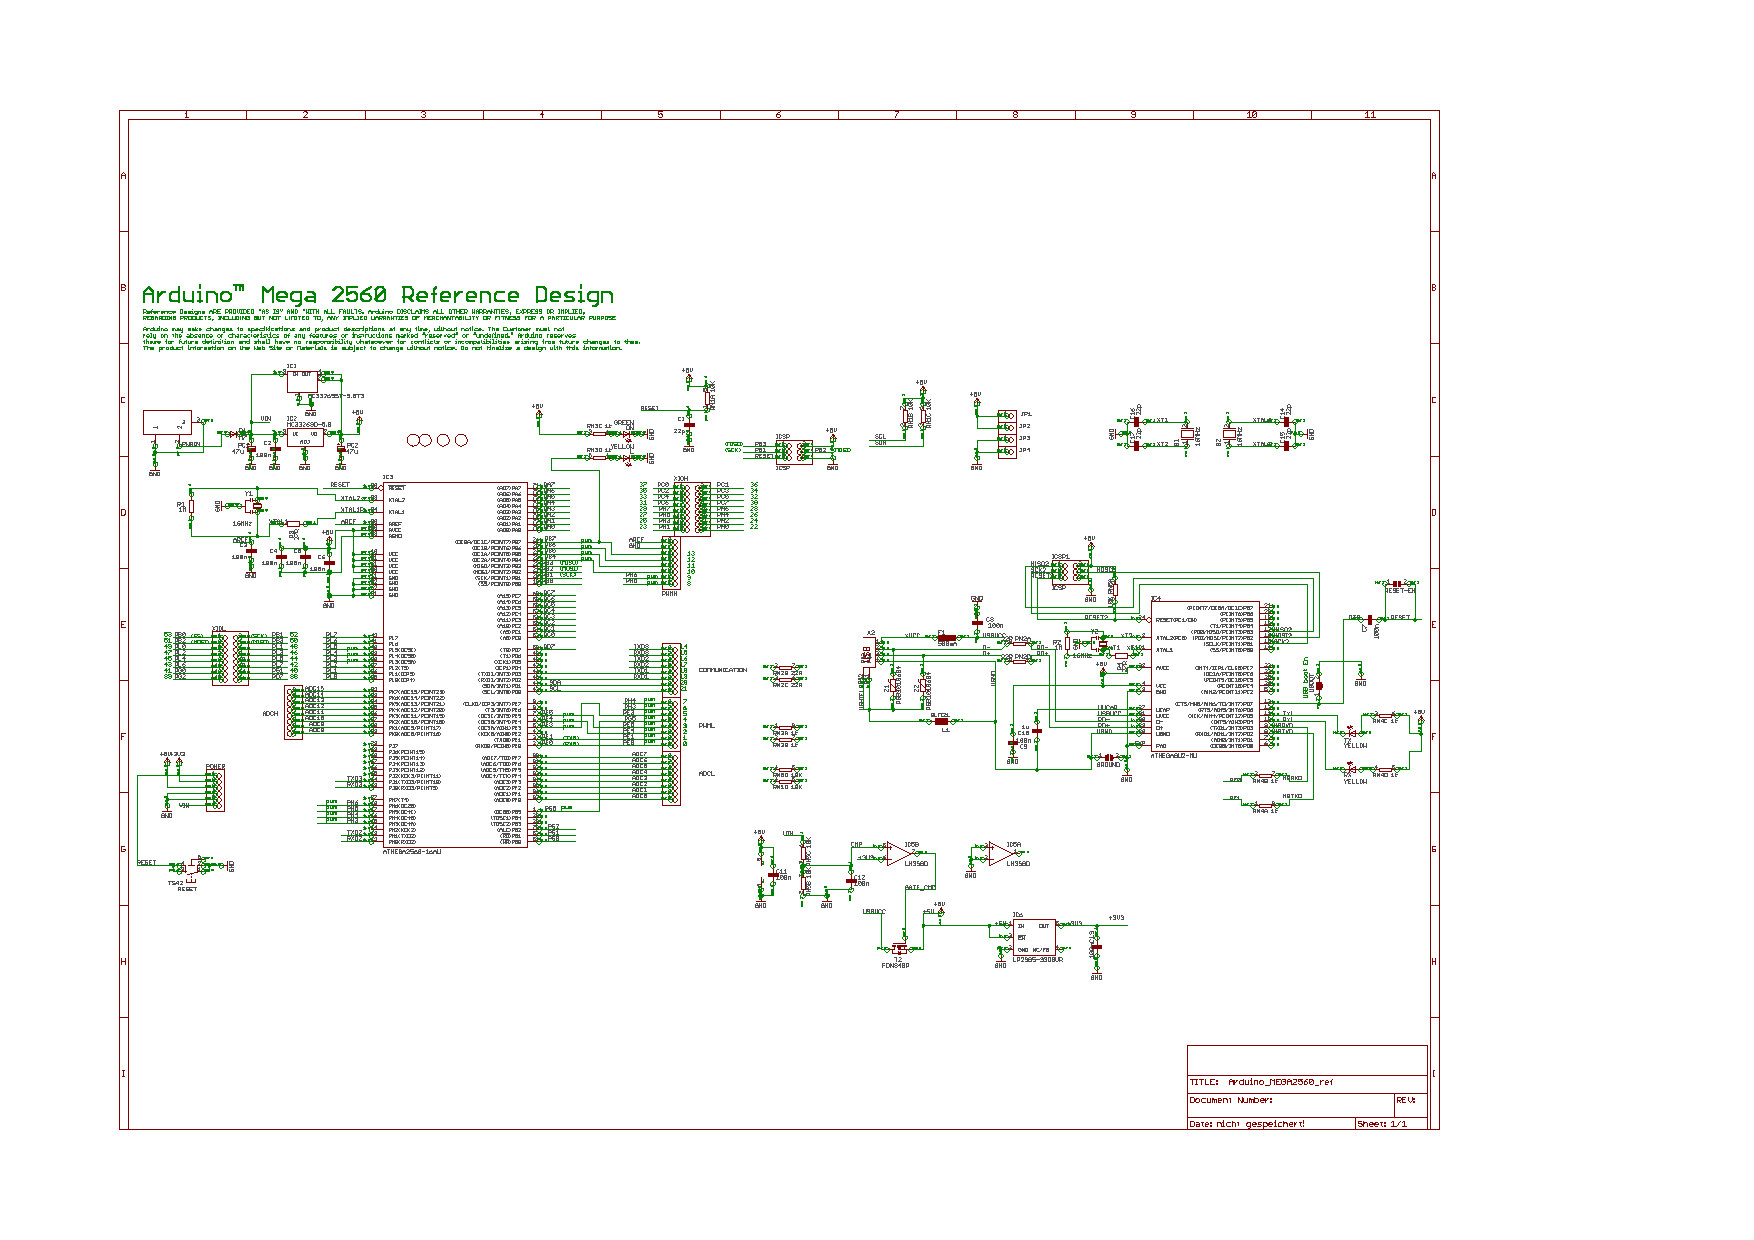
\includepdf[pagecommand={\section{Schaltpläne} \label{sec:Schaltplaene} \subsection{Arduino} \label{sec:sch-Arduino}}, angle=90, scale=0.9]{app/Arduino-sch.pdf}




% Platinenlayout
% --------------

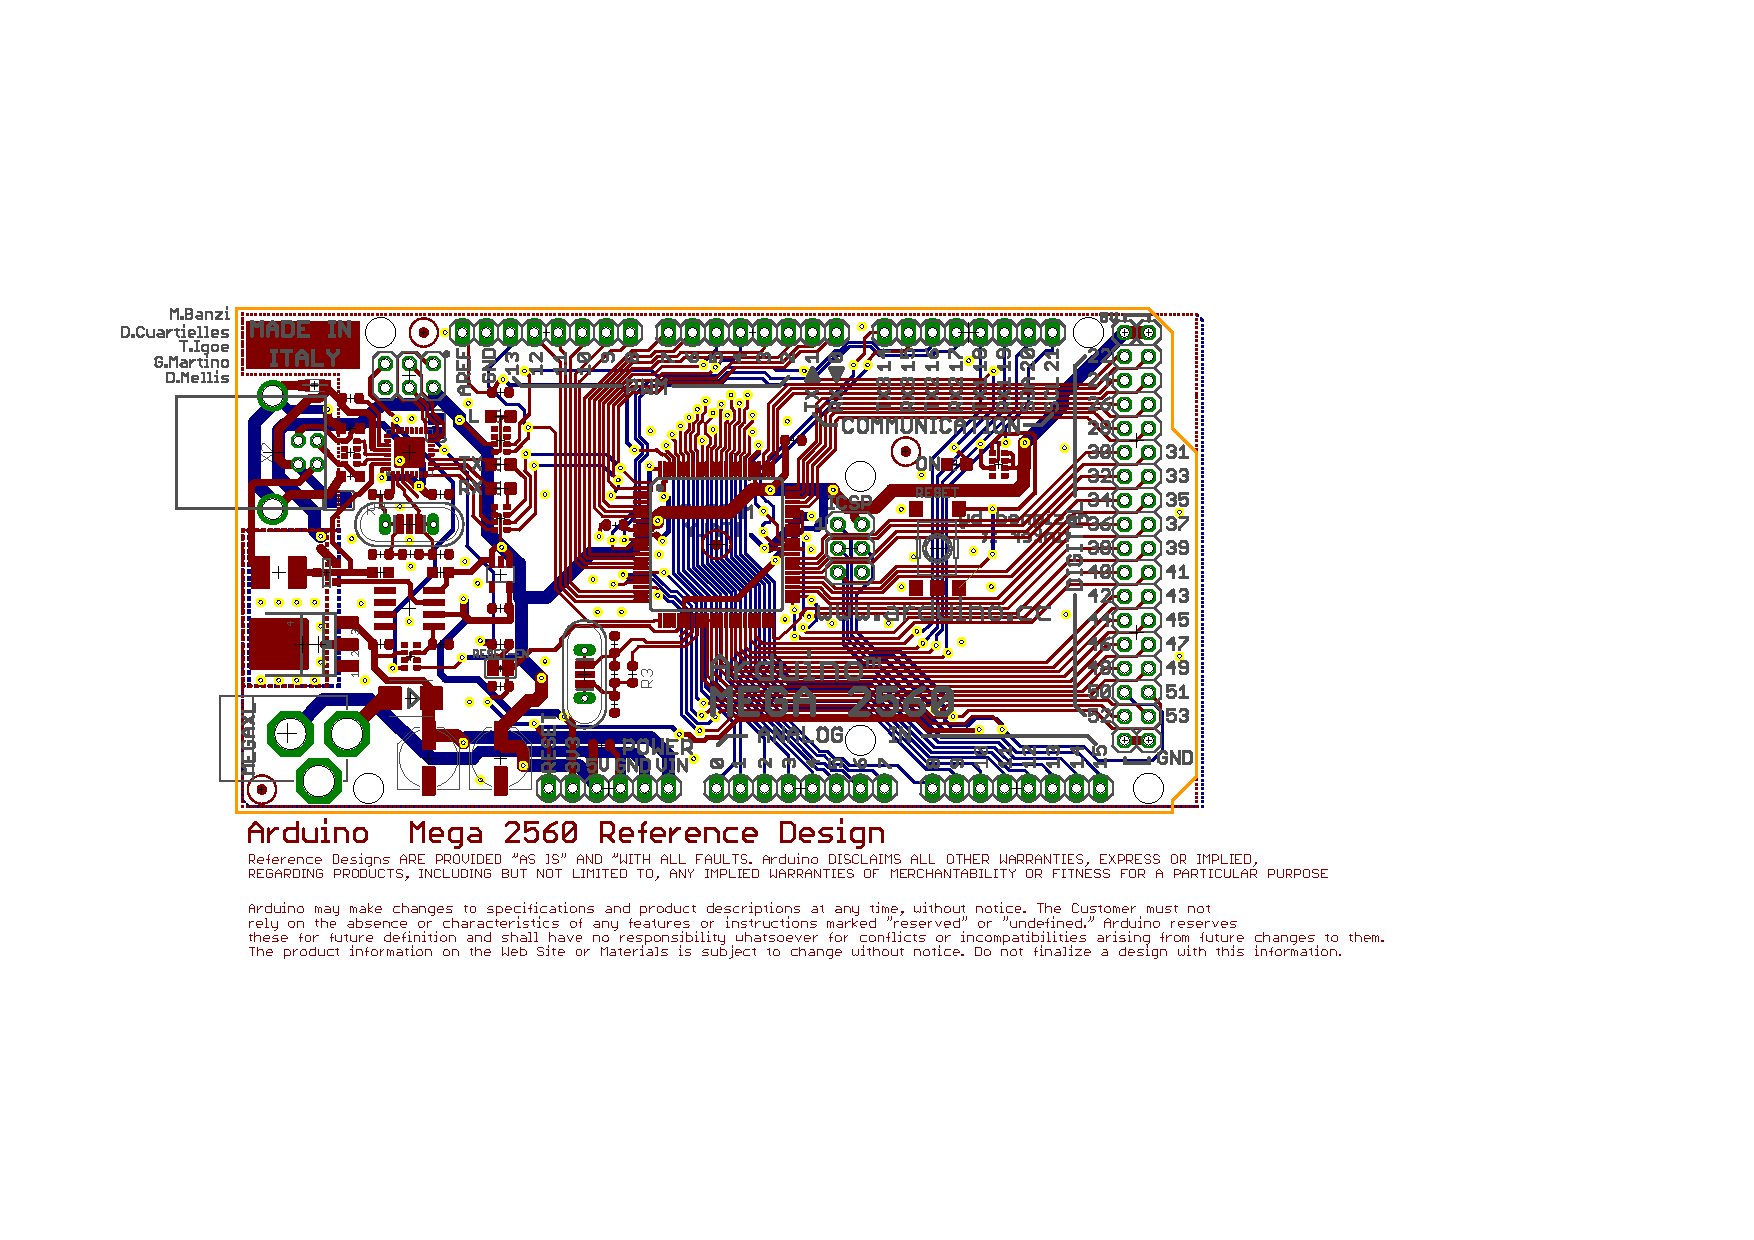
\includepdf[pagecommand={\section{Boardlayouts} \label{sec:Platinenlayout} \subsection{Arduino} \label{sec:brd-Arduino}}, angle=90, scale=1.0]{app/Arduino-brd.pdf}



% Verbindung der Platinen
% -----------------------
%\section{Verbindung der Platinen}



% Messdaten
% ---------
%\section{Messdaten}



% Datenblätter
% ------------
%\section{Datenblätter}



% Inhaltsverzeichnis der beiliegenden CD
% --------------------------------------
\clearpage 
%\includepdf[pagecommand={\section{Inhaltsverzeichnis der beiliegenden CD} \mario{Inhaltsverzeichnis CD fertig machen !}}, scale=0.7]{chapter/InhaltsverzeichnisCd.pdf}

\section{Inhaltsverzeichnis der beiliegenden CD}

\begin{forest}
	for tree={
		font=\ttfamily,
		grow'=0,
		child anchor=west,
		parent anchor=south,
		anchor=west,
		calign=first,
		edge path={
			\noexpand\path [draw, \forestoption{edge}]
			(!u.south west) +(7.5pt,0) |- node[fill,inner sep=1.25pt] {} (.child anchor)\forestoption{edge label};
		},
		before typesetting nodes={
			if n=1
			{insert before={[,phantom]}}
			{}
		},
		fit=band,
		before computing xy={l=15pt},
	}
	[	
		[1-Masterarbeit
			[Abbildungen]
			[Masterarbeit.pdf]
		]
		[2-Hardware
			[Datenblätter]
			[Eagle
				[Schaltung 1]
				[Schaltung 2]
				[\dots]
			]
		]
		[3-Firmware
			[CubeMX
				[Config File 1]
				[\dots]
			]
			[SystemWorkbench
				[Firmware 1]
				[\dots]
			]
		]
		[4-Extras
			[\dots]
		]
	]
\end{forest}


	
% ***********************************************
\end{document}
% ***********************************************
